\chapter{Comparison of Available Datasets}
\label{sec:dataset_selection}

This chapter builds upon the insights elaborated in previous chapters to lay the foundation
for developing a classifier for the \cgls{3L-CVRP} with practical constraints by comparing and
selecting a suitable dataset. The classifier will be used to predict the feasibility of packing a
given set of cuboids into a vehicle - representing a single tour - similar to the approach presented
in Chapter~\ref{sec:motivation_feasibility_prediction} by \citeauthor{zhang_learning-based_2022}.

As discussed in Chapter~\ref{sec:classical_solution_approaches}, the \gls{CLP} is an NP-hard problem,
making it computationally demanding to verify the packing feasibility of individual routes.
A classifier can therefore enhance the performance of existing exact algorithms \footcite[cf.][]{tamke_branch-and-cut_2024}
by reducing the need to compute feasibility exactly - using \cgls{CP} methods - only when a
final solution is found, or just before columns generated in Branch-and-Price or Branch-and-Cut
algorithms are discarded \footcite[cf.][pp. 9--11]{zhang_learning-based_2022}. As many single routes
need to be evaluated this use case has the potential to significantly reduce the overall
computation time. First, several published \cgls{3L-CVRP} datasets will be compared with respect
to their overall characteristics. Subsequently, a more detailed analysis will focus on the
heterogeneity of the items. Finally, a suitable dataset will be selected as a promising foundation
for developing a classifier.

\begin{table}[h]
    \centering
    \small
    \begin{tabular}{@{}lcccc@{}}
        \toprule
        \textbf{Reference}                                  & \textbf{Instances} & \textbf{Customers}  & \textbf{Rel. Mass Range} & \textbf{Orders Range}   \\
        \midrule
        Gendreau, 2006\footcite[cf.][]{gendreau_tabu_2006}  & 27                 & [15, 100]           & [0, 0.91]                & [1, 3]                  \\
        Moura, 2009\footcite[cf.][]{moura_integrated_2009}  & 46                 & 25                  & [0, 0.01]                & [30, 100]               \\
        Ceschia, 2013\footcite[cf.][]{ceschia_local_2013}   & 13                 & [11, 129]           & [0, 0.05]                & [1, 41]                 \\
        Krebs\_a, 2021\footcite[cf.][]{krebs_advanced_2021} & 600                & 20, 60, 100         & [0, 0.58]                & [1, 30]                 \\
        Krebs\_b, 2021\footcite[cf.][]{krebs_axle_2021}     & 80                 & 30, 60, 90, 120     & [0, 0.04]                & [1, 22]                 \\
        \toprule
        \textbf{Reference}                                  & \textbf{Items}     & \textbf{Item Types} & \textbf{Min dimension}   & \textbf{Max dimensions} \\
        \midrule
        Gendreau, 2006                                      & [26, 199]          & [26, 199]           & \{12, 5, 6\}             & \{36, 15, 18\}          \\
        Moura, 2009                                         & 1050, 1550         & 5                   & \{8.1, 3.3, 2.5\}        & \{12, 9.9, 7.3\}        \\
        Ceschia, 2013                                       & [254, 8060]        & [9, 97]             & \{0.1, 0.5, 0.1\}        & \{66, 23, 28.4\}        \\
        Krebs\_a, 2021                                      & 200, 400           & 3, 10, 100          & \{6, 2, 2\}              & \{35, 14, 14\}          \\
        Krebs\_b, 2021                                      & 200, 400           & 10, 100             & \{6, 6, 6\}              & \{25, 12, 15\}          \\
        \bottomrule
    \end{tabular}
    \caption{Numeric comparisons between available datasets.}
    \label{tab:dataset_comparison}
\end{table}
\begin{comment}
\begin{table}[!ht]
    \centering
    \small
    \begin{tabular}{@{}lcccc@{}}
        \toprule
        \textbf{Reference}                                  & \textbf{Instances} & \textbf{Customers}  & \textbf{Rel. Mass Range} & \textbf{Orders Range}   \\
        \midrule
        Gendreau, 2006\footcite[cf.][]{gendreau_tabu_2006}  & 27                 & [15, 100]           & [0, 0.91]                & [1, 3]                  \\
        Moura, 2009\footcite[cf.][]{moura_integrated_2009}  & 46                 & 25                  & [0, 0.01]                & [30, 100]               \\
        Ceschia, 2013\footcite[cf.][]{ceschia_local_2013}   & 13                 & [11, 129]           & [0, 0.05]                & [1, 41]                 \\
        Krebs\_a, 2021\footcite[cf.][]{krebs_advanced_2021} & 600                & \{20, 60, 100\}     & [0, 0.58]                & [1, 30]                 \\
        Krebs\_b, 2021\footcite[cf.][]{krebs_axle_2021}     & 80                 & \{30, 60, 90, 120\} & [0, 0.04]                & [1, 22]                 \\
        \toprule
        \textbf{Reference}                                  & \textbf{Items}     & \textbf{Item Types} & \textbf{Min dimension}   & \textbf{Max dimensions} \\
        \midrule
        Gendreau, 2006                                      & [26, 199]          & [26, 199]           & \{12, 5, 6\}             & \{36, 15, 18\}          \\
        Moura, 2009                                         & \{1050, 1550\}     & 5                   & \{8.1, 3.3, 2.5\}        & \{12, 9.9, 7.3\}        \\
        Ceschia, 2013                                       & [254, 8060]        & [9, 97]             & \{0.1, 0.5, 0.1\}        & \{66, 23, 28.4\}        \\
        Krebs\_a, 2021                                      & \{200, 400\}       & \{3, 10, 100\}      & \{6, 2, 2\}              & \{35, 14, 14\}          \\
        Krebs\_b, 2021                                      & \{200, 400\}       & \{10, 100\}         & \{6, 6, 6\}              & \{25, 12, 15\}          \\
        \bottomrule
    \end{tabular}
    \caption{Numeric comparisons between available datasets.}
    \label{tab:dataset_comparison}
\end{table}
\end{comment}

\begin{figure}[ht]
    \centering
    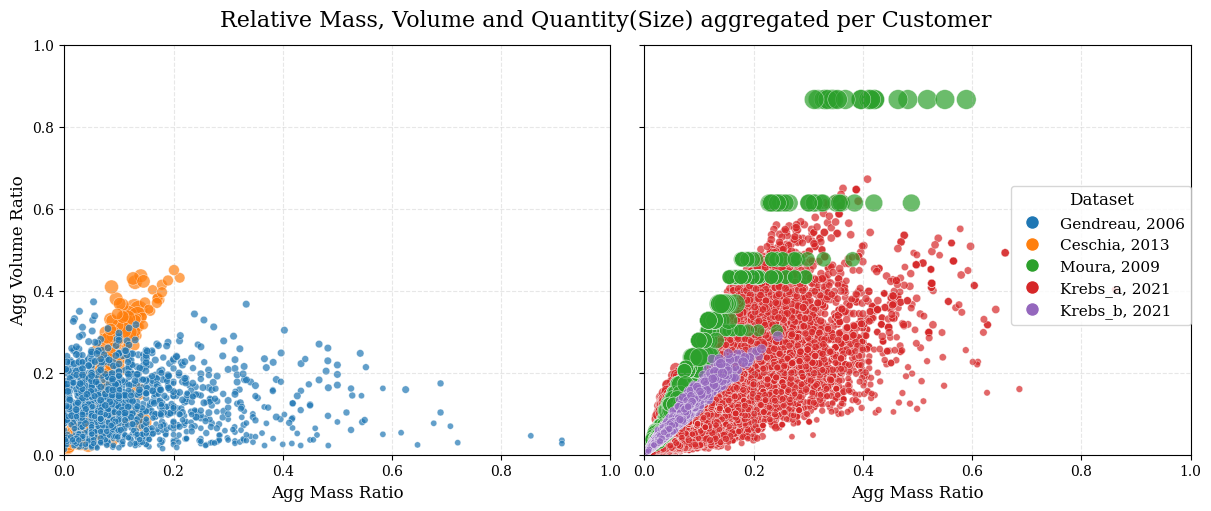
\includegraphics[width=0.8\textwidth]{pictures/comparison_datasets_3lcvrp.png}
    \caption{Visualized 3D packing with packing constraints}.
    \label{fig:dataset_comparison}
\end{figure}


\begin{figure}[ht]
    \centering
    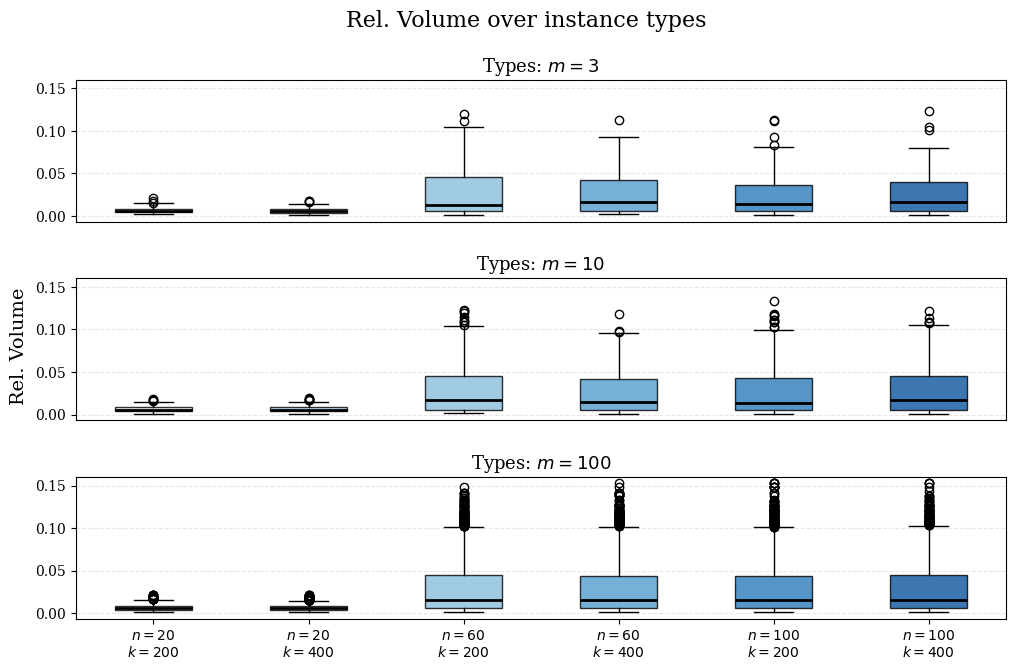
\includegraphics[width=0.8\textwidth]{pictures/volume_over_instances_krebs.png}
    \caption{Visualized 3D packing with packing constraints}.
    \label{fig:krebs_dataset_analysis}
\end{figure}


%\section{Overview of Public Datasets}
%\section{Evaluation Criteria: Diversity, Realism, Labeling, Size}
%\section{Comparison of Selected Datasets}
%\section{Justification for Dataset Selection}